\subsection{Временные ряды}

    На временных рядах можно продемонстрировать как различные виды шумавлияют на поведение системы.

    На рисунке \ref{time_series_x_0_06_a_1_b_0_56} изображено поведениемодели без добавления каких-либо шумов. Видно, что значения переменной \(x\) с течением времени стабилизируются. Численность популяциифактически остается неизменной.

    \begin{figure}
        \centering
        \subfloat[Для модели (\ref{origin})]{
            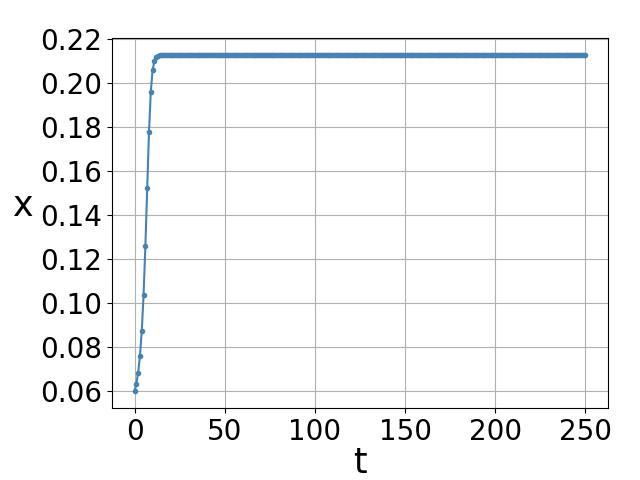
\includegraphics[width=0.5\textwidth]{stochastic/images/time_series_x_0_06_a_1_b_0_56.jpg}
            \label{time_series_x_0_06_a_1_b_0_56}
        }
        \subfloat[Для модели (\ref{alpha_chaos})]{
            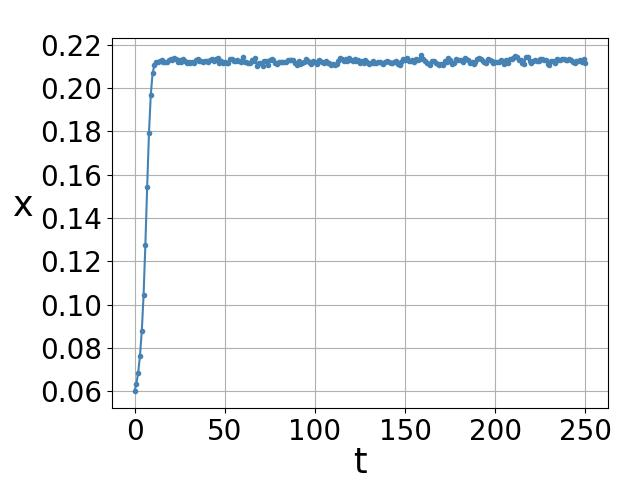
\includegraphics[width=0.5\textwidth]{stochastic/images/time_series_x_0_06_a_1_b_0_56_alpha_chaos_epsilon_0_004.jpg}
            \label{time_series_x_0_06_a_1_b_0_56_alpha_chaos_epsilon_0_004}
        }  

        \subfloat[Для модели (\ref{beta_chaos})]{
            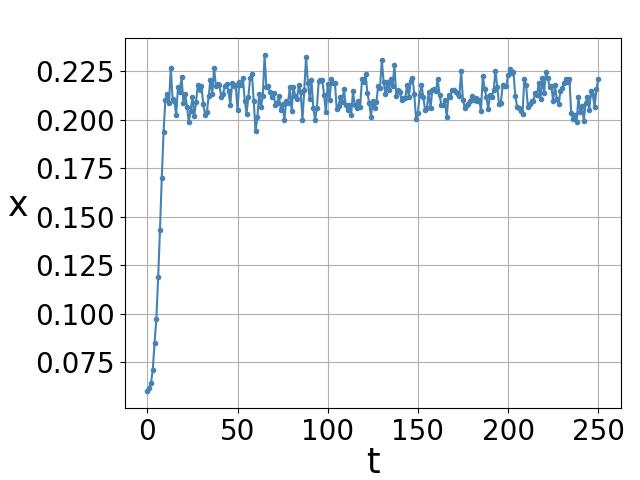
\includegraphics[width=0.5\textwidth]{stochastic/images/time_series_x_0_06_a_1_b_0_56_beta_chaos_epsilon_0_004.jpg}
            \label{time_series_x_0_06_a_1_b_0_56_beta_chaos_epsilon_0_004}
        }
        \subfloat[Для модели (\ref{additive_chaos})]{
            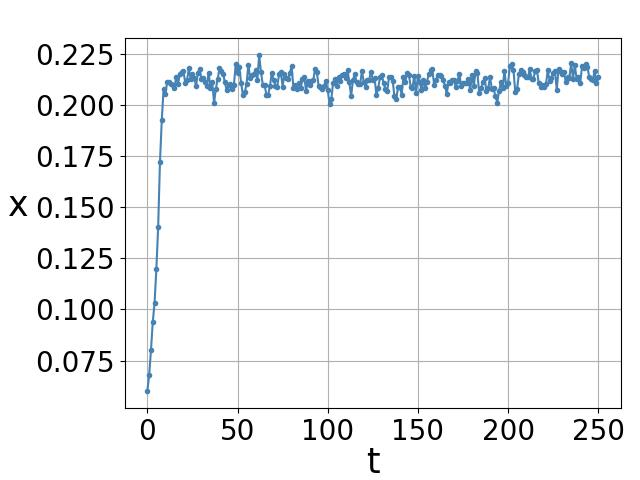
\includegraphics[width=0.5\textwidth]{stochastic/images/time_series_x_0_06_a_1_b_0_56_additive_chaos_epsilon_0_004.jpg}
            \label{time_series_x_0_06_a_1_b_0_56_additive_chaos_epsilon_0_004}
        }
        
        \caption{Временные ряды при \(\alpha = 1, \beta = 0.56, x_0 = 0.06, \varepsilon = 0.004\)}
    \end{figure}

    Далее на рисунках \ref{time_series_x_0_06_a_1_b_0_56_alpha_chaos_epsilon_0_004}, \ref{time_series_x_0_06_a_1_b_0_56_beta_chaos_epsilon_0_004}, \ref{time_series_x_0_06_a_1_b_0_56_additive_chaos_epsilon_0_004} представлены временные ряды для различных видов шума: 

    \begin{enumerate}[a)]
        \setcounter{enumi}{1}
        \item \(\alpha\)-шум
        \item \(\beta\)-шум
        \item аддитивный шум
    \end{enumerate}

    Все варианты рассматриваются с одной и той же интенсивностью шума \(\varepsilon = 0.004\). 
        
    Вид шума влияет на величину разброса значений численности популяции. \comment{Дисперсия?}. И если в модели (\ref{origin}) численность популяции стабилизировалась и переставала хоть сколько-нибудь меняться, то в моделях (\ref{alpha_chaos}), (\ref{beta_chaos}) и (\ref{additive_chaos}) численность постоянно всегда колеблется. Эти колебания происходят в рамках некоторого коридора значений. Численность популяции не растет и не уменьшается на какую-то значительную величину. Но такое поведение наблюдается не всегда.

    \comment{малый шум будет оказывать незначительное влияние, а большой - огромное.}

    \comment{Можно взять оригинальный временной ряд и на него сверху наложить временной ряд с шумом.}

    \comment{Хорошая фраза: индуцированный шумом переход}

    Для демонстрации другого возможного поведения увеличим интенсивность шума. Теперь \(\varepsilon = 0.04\). На графике \ref{time_series_x_0_06_a_1_b_0_56_beta_chaos_epsilon_0_04_fall} видна ситуация, когда шум оказал негативное влияние на численность популяции. Но все не так просто. Если алгоритм, который просчитывает нашу модель, запустить еще раз, то получаем ситуацию, когда популяция выживала на протяжении анализируемого интервала времени. Данный пример проиллюстрирован на картинке \ref{time_series_x_0_06_a_1_b_0_56_beta_chaos_epsilon_0_04_alive}. Аналогичные эффекты можно наблюдать и при других видах шума.

    \comment{Примерно в \(t = 50\) обе популяции были близки к вымиранию, но одна выжила, а вторая нет.}

    \begin{figure}
        \centering
        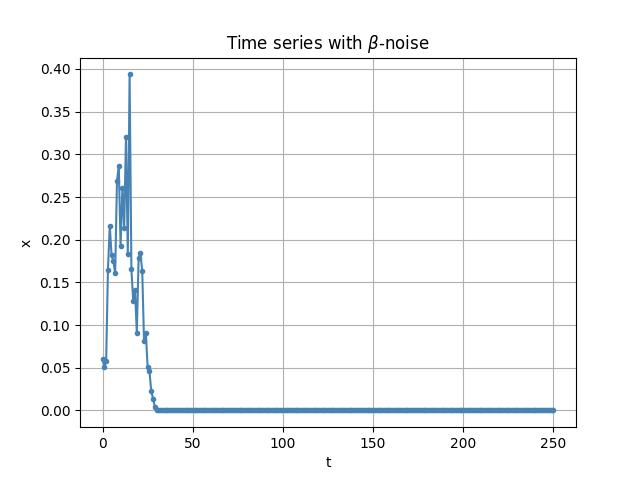
\includegraphics[width=\textwidth]{stochastic/images/time_series_x_0_06_a_1_b_0_56_beta_chaos_epsilon_0_04_fall.jpg}
        
        \captionsetup{justification=centering}
        \caption{Временной ряд модели (\ref{beta_chaos}) при \(\beta = 0.56, \alpha = 1, x_0 = 0.06, \varepsilon = 0.04\)}
        \label{time_series_x_0_06_a_1_b_0_56_beta_chaos_epsilon_0_04_fall}
    \end{figure}

    \begin{figure}
        \centering
        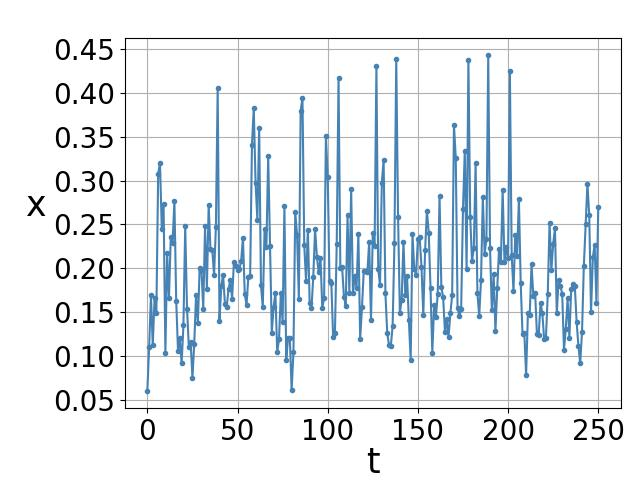
\includegraphics[width=\textwidth]{stochastic/images/time_series_x_0_06_a_1_b_0_56_beta_chaos_epsilon_0_04_alive.jpg}
        
        \captionsetup{justification=centering}
        \caption{Временной ряд модели (\ref{beta_chaos}) при \(\beta = 0.56, \alpha = 1, x_0 = 0.06, \varepsilon = 0.04\)}
        \label{time_series_x_0_06_a_1_b_0_56_beta_chaos_epsilon_0_04_alive}
    \end{figure}

    При добавлении в модель случайных событий ее поведение становится непредсказуемым. Одно незначительное изменение может кардинально повлиять на ход развития событий. 

    \comment{рассматривать как в том семестре все возможные варианты поведения системы в зависимости от начальной точки думаю не надо и так все понятно.}